\chapter{Budget Analysis}
\label{ch:budget}
	
	\section{Project tasks and sheduling}

		\begin{figure}[h]
			\centering
		    	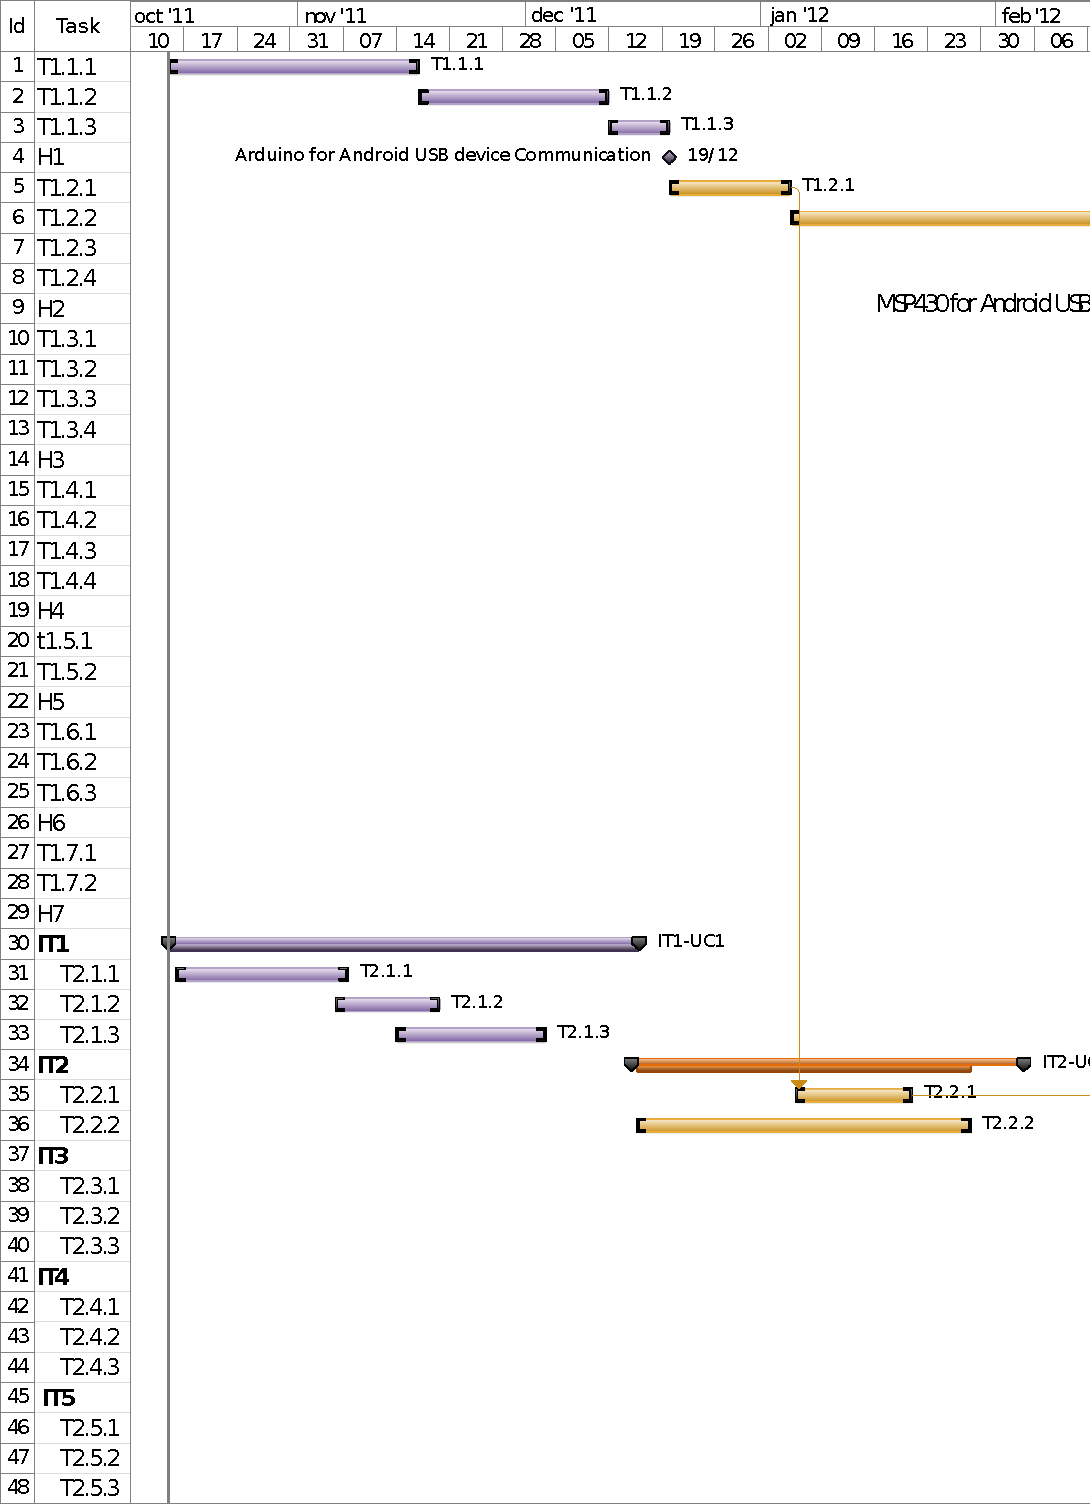
\includegraphics[width=\textwidth]{gantt-l}
			\label{fig:gantL}
		\end{figure}
		\begin{figure}[h]
			\centering
		    	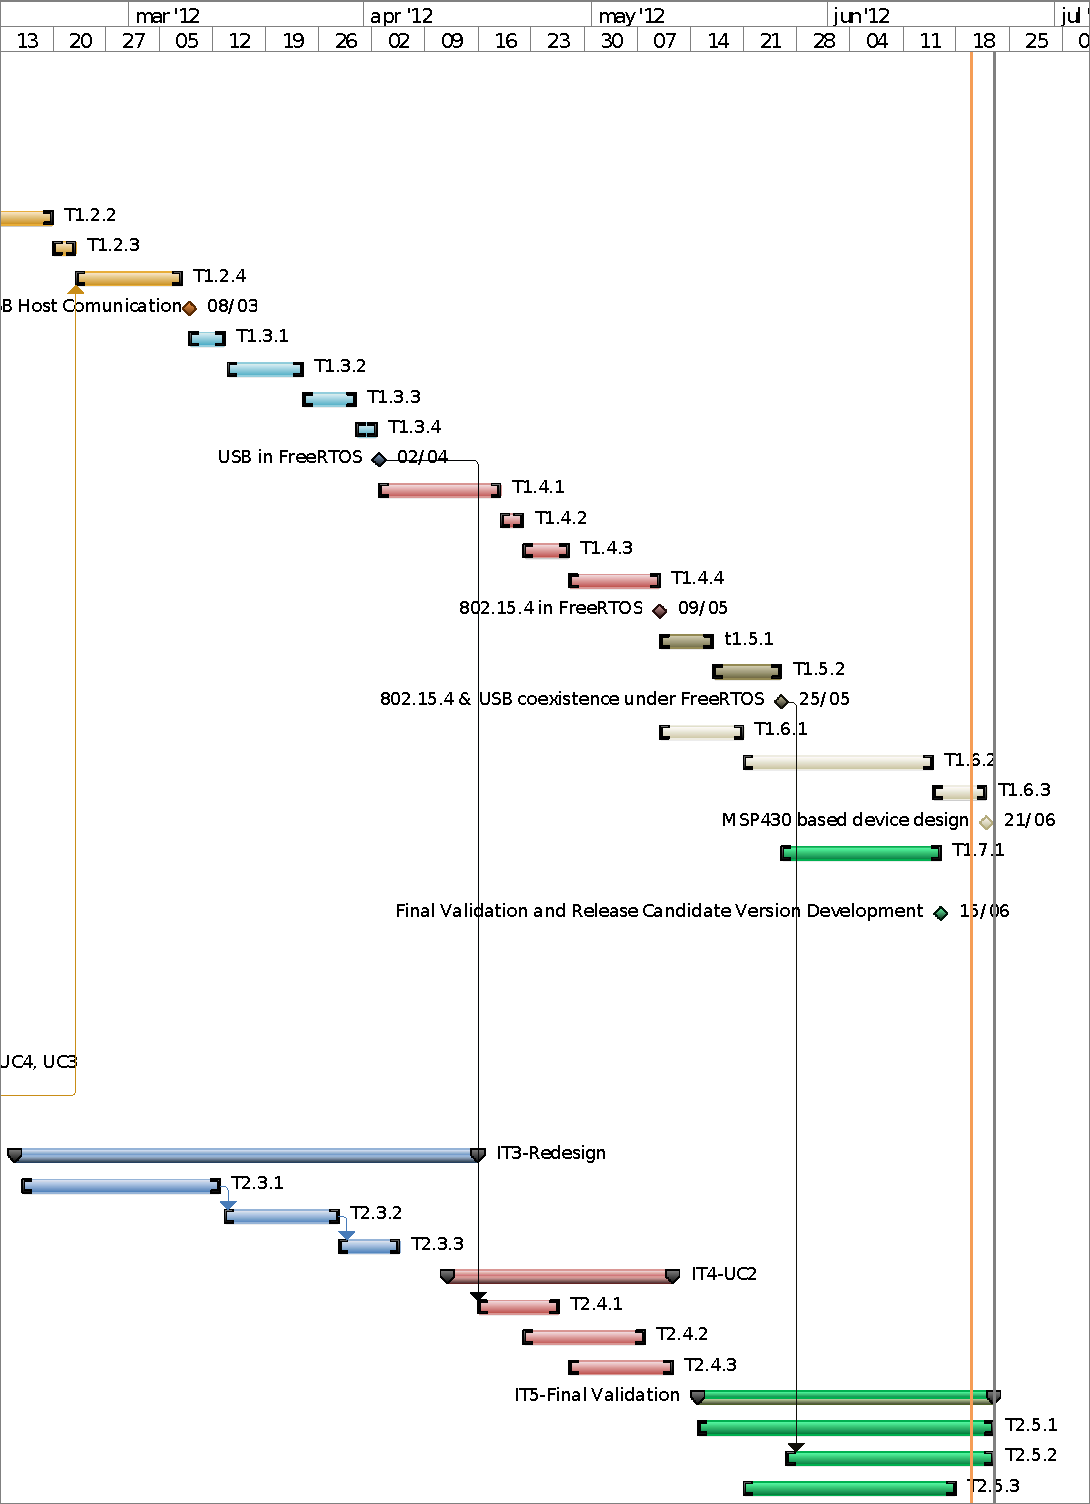
\includegraphics[width=\textwidth]{gantt-r}
			\label{fig:gantR}
		\end{figure}

		\begin{tabular}{| c | p{7cm} | l | l |} % | l | para el hw
		\hline
T1.1.1 & Acquire a suitable Android device prototyping environment & 15/10/2011 & 16/11/2011\\ \hline
T1.1.2 & Manage correct communication between Android and a prototype device & 17/11/2011 & 11/12/2011\\ \hline
T1.1.3 & Develop an application emulating desired behaviour & 12/12/2011 & 19/12/2011\\ \hline
H1 & Arduino for Android USB device Communication & 19/12/2011 & 19/12/2011\\ \hline
T1.2.1 & Supply MSP430 with USB protocol application functionality & 20/12/2011 & 04/01/2012\\ \hline
T1.2.2 & Research Android USB protocol related functionality & 05/01/2012 & 19/02/2012\\ \hline
T1.2.3 & Make Android OS recognize MSP430 when plugged	 & 20/02/2012 & 22/02/2012\\ \hline
T1.2.4 & Manage communication between Android and MSP430 via USB & 23/02/2012 & 07/03/2012\\ \hline
H2 & MSP430 for Android USB Host Comunication & 08/03/2012 & 08/03/2012\\ \hline
T1.3.1 & Check the proper working of FreeRTOS with the new microcontroller & 09/03/2012 & 13/03/2012\\ \hline
T1.3.2 & Validate the feasibility of the usage of USB API along with FreeRTOS in MSP430 & 14/03/2012 & 23/03/2012\\ \hline
T1.3.3 & Correctly integrate USB API into FreeRTOS & 24/03/2012 & 31/03/2012\\ 
\hline
\end{tabular}\\\\

\begin{tabular}{| c | p{6cm} | l | l |} % | l | para el hw
\hline
T1.3.4 & Manage USB data sending in FreeRTOS & 31/03/2012 & 02/04/2012\\ \hline
H3 & USB in FreeRTOS & 02/04/2012 & 02/04/2012\\ \hline
T1.4.1 & Validate current implementation of 802.15.4 in FreeRTOS in MSP430 testing board & 03/04/2012 & 18/04/2012\\ \hline
T1.4.2 & Manage connection to the CC2420 radio module to target MSP430 device & 19/04/2012 & 21/04/2012\\ \hline
T1.4.3 & Port implementation of 802.15.4 to target MSP430 device & 22/04/2012 & 28/04/2012\\ \hline
T1.4.4 & Prepare such implementation for actual usage & 28/04/2012 & 09/05/2012\\ \hline
H4 & 802.15.4 in FreeRTOS & 09/05/2012 & 09/05/2012\\ \hline
t1.5.1 & Assess conflict-free coexistence of current implementation of both USB and 802.15.4 modules in MSP430 & 10/05/2012 & 16/05/2012\\ \hline
T1.5.2 & Manage sending data received from 802.15.4 via USB & 17/05/2012 & 25/05/2012\\ \hline
H5 & 802.15.4 \& USB coexistence under FreeRTOS & 25/05/2012 & 25/05/2012\\ \hline
T1.6.1 & Exhaustive analysis of the reference board & 10/05/2012 & 21/05/2012\\ \hline
T1.6.2 & Capture of the board schematic & 21/05/2012 & 14/06/2012\\ \hline
T1.6.3 & Design and routing of the actual PCB & 15/06/2012 & 21/06/2012\\ \hline
H6 & MSP430 based device design & 21/06/2012 & 21/06/2012\\ \hline
T1.7.1 & Final validation of final aplications with prototyping hardware & 26/05/2012 & 16/06/2012\\ \hline
T1.7.2 & Final validation of final aplications with final hardware & Not performed & Not performed\\ \hline
H7 & Final Validation and Release Candidate Version Development & 15/06/2012 & 15/06/2012\\ \hline
IT1 & Completed UC1 & 15/10/2011 & 15/12/2011\\ \hline
   T2.1.1 & Instruction of the team on Android development & 16/10/2011 & 07/11/2011\\ \hline
   T2.1.2 & Lay out of an initial version of the application architecture & 06/11/2011 & 19/11/2011\\ 
\hline
\end{tabular}\\\\

\begin{tabular}{| c | p{6cm} | l | l |} % | l | para el hw
\hline
   T2.1.3 & Implementation of the Bluetooth receiver module & 14/11/2011 & 03/12/2011\\ \hline
IT2 & Completed UC4, UC3 & 15/12/2011 & 04/02/2012\\ \hline
   T2.2.1 & Development of the USB communication module & 05/01/2012 & 20/01/2012\\ \hline
   T2.2.2 & Implementation of the Log visualization module & 15/12/2011 & 28/01/2012\\ \hline
IT3 & Completed Redesign	15/02/2012 & 15/04/2012\\ \hline
   T2.3.1 & Redesign of the application architecture & 16/02/2012 & 12/03/2012\\ \hline
   T2.3.2 & Achievement of required performance on data management & 13/03/2012 & 28/03/2012\\ \hline
   T2.3.3 & Scheduling of the rest of the project time & 28/03/2012 & 05/04/2012\\ \hline
IT4 & Completed UC2 & 12/04/2012 & 11/05/2012\\ \hline
   T2.4.1 & Implementation of USB host communication & 16/04/2012 & 26/04/2012\\ \hline
   T2.4.2 & Achievement of required performance in rendering & 22/04/2012 & 07/05/2012\\ \hline
   T2.4.3 & Implementation of actual user interfaces & 28/04/2012 & 11/05/2012\\ \hline
IT5 & Final Validation & 15/05/2012 & 22/06/2012\\ \hline
   T2.5.1 & Exhaustive testing of the Android application & 15/05/2012 & 22/06/2012\\ \hline
   T2.5.2 & Validation of the application, the receiver and the delineator node acting as a whole & 26/05/2012 & 22/06/2012\\ \hline
   T2.5.3 & Obtention of the final version of the system by implementing the required amendments identified by the testing procedure. & 21/05/2012 & 17/06/2012\\
\hline
\end{tabular}\\\\


\section{Asset cost}

	A partir de la planificación anterior, que es la real del proyecto, y considerando que hubo en total cerca de dos meses de vacaciones, podemos considerar que este proyecto tiene una duración de 7 meses con 3 personas trabajando a media jornada. Tipicamente el salario de un ingeniero trabajando en este campo sería de unos 35 euros la hora. Por lo que el coste de un ingeniero durante 7 meses a media jornada sería 35euros/hora * 4 horas/dia * 22 dias/mes * 7 meses = 21560\\

	Este coste, unido al de los productos que habría habido que adquirir si no hubiera habido nada en el lugar donde se realizase el proyecto nos dan el coste total del proyecto:\\

\begin{tabular}{| p{5cm} |l | l | l |} 
\hline
   Name & Number& Price per unit & Total price\\ \hline
   Motorola Xoom - Wifi & 1 & 399 & 399\\ \hline
   Google ADK & 1 & 70,8 & 70,8\\ \hline
   Exp430F5438 + MSP430F5438A & 1 & 117,89 & 117,89\\ \hline
   TS430PZ100USB + 2xMSP430F6638 & 1 & 60 & 60\\ \hline
   CC2420 & 1 & 4,00 & 4,00\\ \hline
   Prototype & 1 & 37,662 & 37,662\\ \hline
   Final product & 1 & 41,662 & 41,662\\ \hline
   Enginer & 3 & 21560 & 64680\\ \hline
   Total & & & 65392,13\\ \hline
\hline
\end{tabular}\\\\


\chapter{Product Cost}
\label{ch:cost}

	El coste de fabricar un dispositivo de manera individual, que es lo que se ha hecho durante el proyecto es el siguiente:\\

\begin{tabular}{| c |l | l | l | l |} 
	\hline
		Name & Reference & Number & Price per unit & Total price\\ \hline
		SMT & 1022311 & 2 & 1,96 & 3,92\\ \hline
		Resistor & 1738981 & 2 & 0,062 & 0,124\\ \hline
		LED & 1699413 & 1 & 0,28 & 0,28\\ \hline
		Capacitor & 1833863 & 6 & 0,03 & 0,18\\ \hline
		Capacitor & 1740650 & 2 & 0,154 & 0,308\\ \hline
		Resistor & 1469918 & 1 & 0,038 & 0,038\\ \hline
		Capacitor & 1833865 & 2 & 0,144 & 0,288\\ \hline
		Diode & 1469389 & 3 & 0,099 & 0,297\\ \hline
	   	Capacitor & 1833803 & 1 & 0,085 & 0,085\\ \hline
 		Capacitor & 1327699 & 1 & 0,36 & 0,36 \\ \hline
  		Resistor & 1500615 & 4 & 0,028 & 0,084\\ \hline
	 	Capacitor & 1740632 & 1 & 0,062 & 0,062\\ \hline
	 	MSP430F6638 & 2070274 & 1 & 18,49 & 18,49\\ \hline
	 	Capacitor & 1833888 & 1 & 0,163 & 0,163\\ \hline
	 	Capacitor & 499160 & 2 & 0,122 & 0,244\\ \hline
	 	ESD protection & 1269406 & 1 & 0,63 & 0,63\\ \hline
	 	Microcrystal & 1539364 & 1 & 2,19 & 2,19\\ \hline
	 	Capacitor & 1658880 & 2 & 1,98 & 3,96\\ \hline
	 	MGRID & 1756749 & 8 & 0,057 & 0,456\\ \hline
	 	Header & 7472285 & 1 & 1,34 & 1,34\\ \hline
	 	Milligrid & 511031 & 1 & 0,163 & 0,163\\ \hline
	 	Radio & From TI & 1 & 4,00 & 4,00\\ \hline
	 	Total &  &  &  & 37,662\\ \hline
	\hline
\end{tabular}\\\\
















